\documentclass[12pt]{article}

%packages
%\usepackage{latexsym}
\usepackage{graphicx}
\usepackage{color}
\usepackage{amsmath}
\usepackage{dsfont}
\usepackage{placeins}
\usepackage{amssymb}
\usepackage{wasysym}
\usepackage{abstract}
\usepackage{hyperref}
\usepackage{etoolbox}
\usepackage{datetime}
\usepackage{xcolor}
\usepackage{alphalph}
\settimeformat{ampmtime}

%\usepackage{pstricks,pst-node,pst-tree}

%\usepackage{algpseudocode}
%\usepackage{amsthm}
%\usepackage{hyperref}
%\usepackage{mathrsfs}
%\usepackage{amsfonts}
%\usepackage{bbding}
%\usepackage{listings}
%\usepackage{appendix}
\usepackage[margin=1in]{geometry}
%\geometry{papersize={8.5in,11in},total={6.5in,9in}}
%\usepackage{cancel}
%\usepackage{algorithmic, algorithm}

\makeatletter
\def\maxwidth{ %
  \ifdim\Gin@nat@width>\linewidth
    \linewidth
  \else
    \Gin@nat@width
  \fi
}
\makeatother

\definecolor{fgcolor}{rgb}{0.345, 0.345, 0.345}
\newcommand{\hlnum}[1]{\textcolor[rgb]{0.686,0.059,0.569}{#1}}%
\newcommand{\hlstr}[1]{\textcolor[rgb]{0.192,0.494,0.8}{#1}}%
\newcommand{\hlcom}[1]{\textcolor[rgb]{0.678,0.584,0.686}{\textit{#1}}}%
\newcommand{\hlopt}[1]{\textcolor[rgb]{0,0,0}{#1}}%
\newcommand{\hlstd}[1]{\textcolor[rgb]{0.345,0.345,0.345}{#1}}%
\newcommand{\hlkwa}[1]{\textcolor[rgb]{0.161,0.373,0.58}{\textbf{#1}}}%
\newcommand{\hlkwb}[1]{\textcolor[rgb]{0.69,0.353,0.396}{#1}}%
\newcommand{\hlkwc}[1]{\textcolor[rgb]{0.333,0.667,0.333}{#1}}%
\newcommand{\hlkwd}[1]{\textcolor[rgb]{0.737,0.353,0.396}{\textbf{#1}}}%

\usepackage{framed}
\makeatletter
\newenvironment{kframe}{%
 \def\at@end@of@kframe{}%
 \ifinner\ifhmode%
  \def\at@end@of@kframe{\end{minipage}}%
  \begin{minipage}{\columnwidth}%
 \fi\fi%
 \def\FrameCommand##1{\hskip\@totalleftmargin \hskip-\fboxsep
 \colorbox{shadecolor}{##1}\hskip-\fboxsep
     % There is no \\@totalrightmargin, so:
     \hskip-\linewidth \hskip-\@totalleftmargin \hskip\columnwidth}%
 \MakeFramed {\advance\hsize-\width
   \@totalleftmargin\z@ \linewidth\hsize
   \@setminipage}}%
 {\par\unskip\endMakeFramed%
 \at@end@of@kframe}
\makeatother

\definecolor{shadecolor}{rgb}{.77, .77, .77}
\definecolor{messagecolor}{rgb}{0, 0, 0}
\definecolor{warningcolor}{rgb}{1, 0, 1}
\definecolor{errorcolor}{rgb}{1, 0, 0}
\newenvironment{knitrout}{}{} % an empty environment to be redefined in TeX

\usepackage{alltt}
\usepackage[T1]{fontenc}

\newcommand{\qu}[1]{``#1''}
\newcounter{probnum}
\setcounter{probnum}{1}

%create definition to allow local margin changes
\def\changemargin#1#2{\list{}{\rightmargin#2\leftmargin#1}\item[]}
\let\endchangemargin=\endlist 

%allow equations to span multiple pages
\allowdisplaybreaks

%define colors and color typesetting conveniences
\definecolor{gray}{rgb}{0.5,0.5,0.5}
\definecolor{black}{rgb}{0,0,0}
\definecolor{white}{rgb}{1,1,1}
\definecolor{blue}{rgb}{0.5,0.5,1}
\newcommand{\inblue}[1]{\color{blue}#1 \color{black}}
\definecolor{green}{rgb}{0.133,0.545,0.133}
\newcommand{\ingreen}[1]{\color{green}#1 \color{black}}
\definecolor{yellow}{rgb}{1,1,0}
\newcommand{\inyellow}[1]{\color{yellow}#1 \color{black}}
\definecolor{orange}{rgb}{0.9,0.649,0}
\newcommand{\inorange}[1]{\color{orange}#1 \color{black}}
\definecolor{red}{rgb}{1,0.133,0.133}
\newcommand{\inred}[1]{\color{red}#1 \color{black}}
\definecolor{purple}{rgb}{0.58,0,0.827}
\newcommand{\inpurple}[1]{\color{purple}#1 \color{black}}
\definecolor{backgcode}{rgb}{0.97,0.97,0.8}
\definecolor{Brown}{cmyk}{0,0.81,1,0.60}
\definecolor{OliveGreen}{cmyk}{0.64,0,0.95,0.40}
\definecolor{CadetBlue}{cmyk}{0.62,0.57,0.23,0}

%define new math operators
\DeclareMathOperator*{\argmax}{arg\,max~}
\DeclareMathOperator*{\argmin}{arg\,min~}
\DeclareMathOperator*{\argsup}{arg\,sup~}
\DeclareMathOperator*{\arginf}{arg\,inf~}
\DeclareMathOperator*{\convolution}{\text{\Huge{$\ast$}}}
\newcommand{\infconv}[2]{\convolution^\infty_{#1 = 1} #2}
%true functions

%%%% GENERAL SHORTCUTS

%shortcuts for pure typesetting conveniences
\newcommand{\bv}[1]{\boldsymbol{#1}}

%shortcuts for compound constants
\newcommand{\BetaDistrConst}{\dfrac{\Gamma(\alpha + \beta)}{\Gamma(\alpha)\Gamma(\beta)}}
\newcommand{\NormDistrConst}{\dfrac{1}{\sqrt{2\pi\sigma^2}}}

%shortcuts for conventional symbols
\newcommand{\tsq}{\tau^2}
\newcommand{\tsqh}{\hat{\tau}^2}
\newcommand{\sigsq}{\sigma^2}
\newcommand{\sigsqsq}{\parens{\sigma^2}^2}
\newcommand{\sigsqovern}{\dfrac{\sigsq}{n}}
\newcommand{\tausq}{\tau^2}
\newcommand{\tausqalpha}{\tau^2_\alpha}
\newcommand{\tausqbeta}{\tau^2_\beta}
\newcommand{\tausqsigma}{\tau^2_\sigma}
\newcommand{\betasq}{\beta^2}
\newcommand{\sigsqvec}{\bv{\sigma}^2}
\newcommand{\sigsqhat}{\hat{\sigma}^2}
\newcommand{\sigsqhatmlebayes}{\sigsqhat_{\text{Bayes, MLE}}}
\newcommand{\sigsqhatmle}[1]{\sigsqhat_{#1, \text{MLE}}}
\newcommand{\bSigma}{\bv{\Sigma}}
\newcommand{\bSigmainv}{\bSigma^{-1}}
\newcommand{\thetavec}{\bv{\theta}}
\newcommand{\thetahat}{\hat{\theta}}
\newcommand{\thetahatmle}{\hat{\theta}_{\mathrm{MLE}}}
\newcommand{\thetavechatmle}{\hat{\thetavec}_{\mathrm{MLE}}}
\newcommand{\muhat}{\hat{\mu}}
\newcommand{\musq}{\mu^2}
\newcommand{\muvec}{\bv{\mu}}
\newcommand{\muhatmle}{\muhat_{\text{MLE}}}
\newcommand{\lambdahat}{\hat{\lambda}}
\newcommand{\lambdahatmle}{\lambdahat_{\text{MLE}}}
\newcommand{\etavec}{\bv{\eta}}
\newcommand{\alphavec}{\bv{\alpha}}
\newcommand{\minimaxdec}{\delta^*_{\mathrm{mm}}}
\newcommand{\ybar}{\bar{y}}
\newcommand{\xbar}{\bar{x}}
\newcommand{\Xbar}{\bar{X}}
\newcommand{\phat}{\hat{p}}
\newcommand{\Phat}{\hat{P}}
\newcommand{\Zbar}{\bar{Z}}
\newcommand{\iid}{~{\buildrel iid \over \sim}~}
\newcommand{\inddist}{~{\buildrel ind \over \sim}~}
\newcommand{\approxdist}{~{\buildrel approx \over \sim}~}
\newcommand{\equalsindist}{~{\buildrel d \over =}~}
\newcommand{\loglik}[1]{\ell\parens{#1}}
\newcommand{\thetahatkminone}{\thetahat^{(k-1)}}
\newcommand{\thetahatkplusone}{\thetahat^{(k+1)}}
\newcommand{\thetahatk}{\thetahat^{(k)}}
\newcommand{\half}{\frac{1}{2}}
\newcommand{\third}{\frac{1}{3}}
\newcommand{\twothirds}{\frac{2}{3}}
\newcommand{\fourth}{\frac{1}{4}}
\newcommand{\fifth}{\frac{1}{5}}
\newcommand{\sixth}{\frac{1}{6}}

%shortcuts for vector and matrix notation
\newcommand{\A}{\bv{A}}
\newcommand{\At}{\A^T}
\newcommand{\Ainv}{\inverse{\A}}
\newcommand{\B}{\bv{B}}
\newcommand{\K}{\bv{K}}
\newcommand{\Kt}{\K^T}
\newcommand{\Kinv}{\inverse{K}}
\newcommand{\Kinvt}{(\Kinv)^T}
\newcommand{\M}{\bv{M}}
\newcommand{\Bt}{\B^T}
\newcommand{\Q}{\bv{Q}}
\newcommand{\Qt}{\Q^T}
\newcommand{\R}{\bv{R}}
\newcommand{\Rt}{\R^T}
\newcommand{\Z}{\bv{Z}}
\newcommand{\X}{\bv{X}}
\newcommand{\Xsub}{\X_{\text{(sub)}}}
\newcommand{\Xsubadj}{\X_{\text{(sub,adj)}}}
\newcommand{\I}{\bv{I}}
\newcommand{\Y}{\bv{Y}}
\newcommand{\sigsqI}{\sigsq\I}
\renewcommand{\P}{\bv{P}}
\newcommand{\Psub}{\P_{\text{(sub)}}}
\newcommand{\Pt}{\P^T}
\newcommand{\Pii}{P_{ii}}
\newcommand{\Pij}{P_{ij}}
\newcommand{\IminP}{(\I-\P)}
\newcommand{\Xt}{\bv{X}^T}
\newcommand{\XtX}{\Xt\X}
\newcommand{\XtXinv}{\parens{\Xt\X}^{-1}}
\newcommand{\XtXinvXt}{\XtXinv\Xt}
\newcommand{\XXtXinvXt}{\X\XtXinvXt}
\newcommand{\x}{\bv{x}}
\newcommand{\onevec}{\bv{1}}
\newcommand{\oneton}{1, \ldots, n}
\newcommand{\yoneton}{y_1, \ldots, y_n}
\newcommand{\yonetonorder}{y_{(1)}, \ldots, y_{(n)}}
\newcommand{\Yoneton}{Y_1, \ldots, Y_n}
\newcommand{\iinoneton}{i \in \braces{\oneton}}
\newcommand{\onetom}{1, \ldots, m}
\newcommand{\jinonetom}{j \in \braces{\onetom}}
\newcommand{\xoneton}{x_1, \ldots, x_n}
\newcommand{\Xoneton}{X_1, \ldots, X_n}
\newcommand{\xt}{\x^T}
\newcommand{\y}{\bv{y}}
\newcommand{\yt}{\y^T}
\renewcommand{\c}{\bv{c}}
\newcommand{\ct}{\c^T}
\newcommand{\tstar}{\bv{t}^*}
\renewcommand{\u}{\bv{u}}
\renewcommand{\v}{\bv{v}}
\renewcommand{\a}{\bv{a}}
\newcommand{\s}{\bv{s}}
\newcommand{\yadj}{\y_{\text{(adj)}}}
\newcommand{\xjadj}{\x_{j\text{(adj)}}}
\newcommand{\xjadjM}{\x_{j \perp M}}
\newcommand{\yhat}{\hat{\y}}
\newcommand{\yhatsub}{\yhat_{\text{(sub)}}}
\newcommand{\yhatstar}{\yhat^*}
\newcommand{\yhatstarnew}{\yhatstar_{\text{new}}}
\newcommand{\z}{\bv{z}}
\newcommand{\zt}{\z^T}
\newcommand{\bb}{\bv{b}}
\newcommand{\bbt}{\bb^T}
\newcommand{\bbeta}{\bv{\beta}}
\newcommand{\beps}{\bv{\epsilon}}
\newcommand{\bepst}{\beps^T}
\newcommand{\e}{\bv{e}}
\newcommand{\Mofy}{\M(\y)}
\newcommand{\KofAlpha}{K(\alpha)}
\newcommand{\ellset}{\mathcal{L}}
\newcommand{\oneminalph}{1-\alpha}
\newcommand{\SSE}{\text{SSE}}
\newcommand{\SSEsub}{\text{SSE}_{\text{(sub)}}}
\newcommand{\MSE}{\text{MSE}}
\newcommand{\RMSE}{\text{RMSE}}
\newcommand{\SSR}{\text{SSR}}
\newcommand{\SST}{\text{SST}}
\newcommand{\JSest}{\delta_{\text{JS}}(\x)}
\newcommand{\Bayesest}{\delta_{\text{Bayes}}(\x)}
\newcommand{\EmpBayesest}{\delta_{\text{EmpBayes}}(\x)}
\newcommand{\BLUPest}{\delta_{\text{BLUP}}}
\newcommand{\MLEest}[1]{\hat{#1}_{\text{MLE}}}

%shortcuts for Linear Algebra stuff (i.e. vectors and matrices)
\newcommand{\twovec}[2]{\bracks{\begin{array}{c} #1 \\ #2 \end{array}}}
\newcommand{\threevec}[3]{\bracks{\begin{array}{c} #1 \\ #2 \\ #3 \end{array}}}
\newcommand{\fivevec}[5]{\bracks{\begin{array}{c} #1 \\ #2 \\ #3 \\ #4 \\ #5 \end{array}}}
\newcommand{\twobytwomat}[4]{\bracks{\begin{array}{cc} #1 & #2 \\ #3 & #4 \end{array}}}
\newcommand{\threebytwomat}[6]{\bracks{\begin{array}{cc} #1 & #2 \\ #3 & #4 \\ #5 & #6 \end{array}}}

%shortcuts for conventional compound symbols
\newcommand{\thetainthetas}{\theta \in \Theta}
\newcommand{\reals}{\mathbb{R}}
\newcommand{\complexes}{\mathbb{C}}
\newcommand{\rationals}{\mathbb{Q}}
\newcommand{\integers}{\mathbb{Z}}
\newcommand{\naturals}{\mathbb{N}}
\newcommand{\forallninN}{~~\forall n \in \naturals}
\newcommand{\forallxinN}[1]{~~\forall #1 \in \reals}
\newcommand{\matrixdims}[2]{\in \reals^{\,#1 \times #2}}
\newcommand{\inRn}[1]{\in \reals^{\,#1}}
\newcommand{\mathimplies}{\quad\Rightarrow\quad}
\newcommand{\mathlogicequiv}{\quad\Leftrightarrow\quad}
\newcommand{\eqncomment}[1]{\quad \text{(#1)}}
\newcommand{\limitn}{\lim_{n \rightarrow \infty}}
\newcommand{\limitN}{\lim_{N \rightarrow \infty}}
\newcommand{\limitd}{\lim_{d \rightarrow \infty}}
\newcommand{\limitt}{\lim_{t \rightarrow \infty}}
\newcommand{\limitsupn}{\limsup_{n \rightarrow \infty}~}
\newcommand{\limitinfn}{\liminf_{n \rightarrow \infty}~}
\newcommand{\limitk}{\lim_{k \rightarrow \infty}}
\newcommand{\limsupn}{\limsup_{n \rightarrow \infty}}
\newcommand{\limsupk}{\limsup_{k \rightarrow \infty}}
\newcommand{\floor}[1]{\left\lfloor #1 \right\rfloor}
\newcommand{\ceil}[1]{\left\lceil #1 \right\rceil}

%shortcuts for environments
\newcommand{\beqn}{\vspace{-0.25cm}\begin{eqnarray*}}
\newcommand{\eeqn}{\end{eqnarray*}}
\newcommand{\bneqn}{\vspace{-0.25cm}\begin{eqnarray}}
\newcommand{\eneqn}{\end{eqnarray}}

%shortcuts for mini environments
\newcommand{\parens}[1]{\left(#1\right)}
\newcommand{\squared}[1]{\parens{#1}^2}
\newcommand{\tothepow}[2]{\parens{#1}^{#2}}
\newcommand{\prob}[1]{\mathbb{P}\parens{#1}}
\newcommand{\cprob}[2]{\prob{#1~|~#2}}
\newcommand{\littleo}[1]{o\parens{#1}}
\newcommand{\bigo}[1]{O\parens{#1}}
\newcommand{\Lp}[1]{\mathbb{L}^{#1}}
\renewcommand{\arcsin}[1]{\text{arcsin}\parens{#1}}
\newcommand{\prodonen}[2]{\bracks{\prod_{#1=1}^n #2}}
\newcommand{\mysum}[4]{\sum_{#1=#2}^{#3} #4}
\newcommand{\sumonen}[2]{\sum_{#1=1}^n #2}
\newcommand{\infsum}[2]{\sum_{#1=1}^\infty #2}
\newcommand{\infprod}[2]{\prod_{#1=1}^\infty #2}
\newcommand{\infunion}[2]{\bigcup_{#1=1}^\infty #2}
\newcommand{\infinter}[2]{\bigcap_{#1=1}^\infty #2}
\newcommand{\infintegral}[2]{\int^\infty_{-\infty} #2 ~\text{d}#1}
\newcommand{\supthetas}[1]{\sup_{\thetainthetas}\braces{#1}}
\newcommand{\bracks}[1]{\left[#1\right]}
\newcommand{\braces}[1]{\left\{#1\right\}}
\newcommand{\set}[1]{\left\{#1\right\}}
\newcommand{\abss}[1]{\left|#1\right|}
\newcommand{\norm}[1]{\left|\left|#1\right|\right|}
\newcommand{\normsq}[1]{\norm{#1}^2}
\newcommand{\inverse}[1]{\parens{#1}^{-1}}
\newcommand{\rowof}[2]{\parens{#1}_{#2\cdot}}

%shortcuts for functionals
\newcommand{\realcomp}[1]{\text{Re}\bracks{#1}}
\newcommand{\imagcomp}[1]{\text{Im}\bracks{#1}}
\newcommand{\range}[1]{\text{range}\bracks{#1}}
\newcommand{\colsp}[1]{\text{colsp}\bracks{#1}}
\newcommand{\rowsp}[1]{\text{rowsp}\bracks{#1}}
\newcommand{\tr}[1]{\text{tr}\bracks{#1}}
\newcommand{\rank}[1]{\text{rank}\bracks{#1}}
\newcommand{\proj}[2]{\text{Proj}_{#1}\bracks{#2}}
\newcommand{\projcolspX}[1]{\text{Proj}_{\colsp{\X}}\bracks{#1}}
\newcommand{\median}[1]{\text{median}\bracks{#1}}
\newcommand{\mean}[1]{\text{mean}\bracks{#1}}
\newcommand{\dime}[1]{\text{dim}\bracks{#1}}
\renewcommand{\det}[1]{\text{det}\bracks{#1}}
\newcommand{\expe}[1]{\mathbb{E}\bracks{#1}}
\newcommand{\expeabs}[1]{\expe{\abss{#1}}}
\newcommand{\expesub}[2]{\mathbb{E}_{#1}\bracks{#2}}
\newcommand{\indic}[1]{\mathds{1}_{#1}}
\newcommand{\var}[1]{\mathbb{V}\text{ar}\bracks{#1}}
\newcommand{\cov}[2]{\mathbb{C}\text{ov}\bracks{#1, #2}}
\newcommand{\corr}[2]{\text{Corr}\bracks{#1, #2}}
\newcommand{\se}[1]{\mathbb{S}\text{E}\bracks{#1}}
\newcommand{\seest}[1]{\hat{\mathbb{S}\text{E}}\bracks{#1}}
\newcommand{\bias}[1]{\text{Bias}\bracks{#1}}
\newcommand{\derivop}[2]{\dfrac{\text{d}}{\text{d} #1}\bracks{#2}}
\newcommand{\partialop}[2]{\dfrac{\partial}{\partial #1}\bracks{#2}}
\newcommand{\secpartialop}[2]{\dfrac{\partial^2}{\partial #1^2}\bracks{#2}}
\newcommand{\mixpartialop}[3]{\dfrac{\partial^2}{\partial #1 \partial #2}\bracks{#3}}

%shortcuts for functions
\renewcommand{\exp}[1]{\mathrm{exp}\parens{#1}}
\renewcommand{\cos}[1]{\text{cos}\parens{#1}}
\renewcommand{\sin}[1]{\text{sin}\parens{#1}}
\newcommand{\sign}[1]{\text{sign}\parens{#1}}
\newcommand{\are}[1]{\mathrm{ARE}\parens{#1}}
\newcommand{\natlog}[1]{\ln\parens{#1}}
\newcommand{\oneover}[1]{\frac{1}{#1}}
\newcommand{\overtwo}[1]{\frac{#1}{2}}
\newcommand{\overn}[1]{\frac{#1}{n}}
\newcommand{\oneoversqrt}[1]{\oneover{\sqrt{#1}}}
\newcommand{\sqd}[1]{\parens{#1}^2}
\newcommand{\loss}[1]{\ell\parens{\theta, #1}}
\newcommand{\losstwo}[2]{\ell\parens{#1, #2}}
\newcommand{\cf}{\phi(t)}

%English language specific shortcuts
\newcommand{\ie}{\textit{i.e.} }
\newcommand{\AKA}{\textit{AKA} }
\renewcommand{\iff}{\textit{iff}}
\newcommand{\eg}{\textit{e.g.} }
\newcommand{\st}{\textit{s.t.} }
\newcommand{\wrt}{\textit{w.r.t.} }
\newcommand{\mathst}{~~\text{\st}~~}
\newcommand{\mathand}{~~\text{and}~~}
\newcommand{\ala}{\textit{a la} }
\newcommand{\ppp}{posterior predictive p-value}
\newcommand{\dd}{dataset-to-dataset}

%shortcuts for distribution titles
\newcommand{\logistic}[2]{\mathrm{Logistic}\parens{#1,\,#2}}
\newcommand{\bernoulli}[1]{\mathrm{Bernoulli}\parens{#1}}
\newcommand{\betanot}[2]{\mathrm{Beta}\parens{#1,\,#2}}
\newcommand{\stdbetanot}{\betanot{\alpha}{\beta}}
\newcommand{\multnormnot}[3]{\mathcal{N}_{#1}\parens{#2,\,#3}}
\newcommand{\normnot}[2]{\mathcal{N}\parens{#1,\,#2}}
\newcommand{\classicnormnot}{\normnot{\mu}{\sigsq}}
\newcommand{\stdnormnot}{\normnot{0}{1}}
\newcommand{\uniformdiscrete}[1]{\mathrm{Uniform}\parens{\braces{#1}}}
\newcommand{\uniform}[2]{\mathrm{U}\parens{#1,\,#2}}
\newcommand{\stduniform}{\uniform{0}{1}}
\newcommand{\geometric}[1]{\mathrm{Geometric}\parens{#1}}
\newcommand{\hypergeometric}[3]{\mathrm{Hypergeometric}\parens{#1,\,#2,\,#3}}
\newcommand{\exponential}[1]{\mathrm{Exp}\parens{#1}}
\newcommand{\gammadist}[2]{\mathrm{Gamma}\parens{#1, #2}}
\newcommand{\poisson}[1]{\mathrm{Poisson}\parens{#1}}
\newcommand{\binomial}[2]{\mathrm{Binomial}\parens{#1,\,#2}}
\newcommand{\negbin}[2]{\mathrm{NegBin}\parens{#1,\,#2}}
\newcommand{\rayleigh}[1]{\mathrm{Rayleigh}\parens{#1}}
\newcommand{\multinomial}[2]{\mathrm{Multinomial}\parens{#1,\,#2}}
\newcommand{\gammanot}[2]{\mathrm{Gamma}\parens{#1,\,#2}}
\newcommand{\cauchynot}[2]{\text{Cauchy}\parens{#1,\,#2}}
\newcommand{\invchisqnot}[1]{\text{Inv}\chisq{#1}}
\newcommand{\invscaledchisqnot}[2]{\text{ScaledInv}\ncchisq{#1}{#2}}
\newcommand{\invgammanot}[2]{\text{InvGamma}\parens{#1,\,#2}}
\newcommand{\chisq}[1]{\chi^2_{#1}}
\newcommand{\ncchisq}[2]{\chi^2_{#1}\parens{#2}}
\newcommand{\ncF}[3]{F_{#1,#2}\parens{#3}}

%shortcuts for PDF's of common distributions
\newcommand{\logisticpdf}[3]{\oneover{#3}\dfrac{\exp{-\dfrac{#1 - #2}{#3}}}{\parens{1+\exp{-\dfrac{#1 - #2}{#3}}}^2}}
\newcommand{\betapdf}[3]{\dfrac{\Gamma(#2 + #3)}{\Gamma(#2)\Gamma(#3)}#1^{#2-1} (1-#1)^{#3-1}}
\newcommand{\normpdf}[3]{\frac{1}{\sqrt{2\pi#3}}\exp{-\frac{1}{2#3}(#1 - #2)^2}}
\newcommand{\normpdfvarone}[2]{\dfrac{1}{\sqrt{2\pi}}e^{-\half(#1 - #2)^2}}
\newcommand{\chisqpdf}[2]{\dfrac{1}{2^{#2/2}\Gamma(#2/2)}\; {#1}^{#2/2-1} e^{-#1/2}}
\newcommand{\invchisqpdf}[2]{\dfrac{2^{-\overtwo{#1}}}{\Gamma(#2/2)}\,{#1}^{-\overtwo{#2}-1}  e^{-\oneover{2 #1}}}
\newcommand{\exponentialpdf}[2]{#2\exp{-#2#1}}
\newcommand{\poissonpdf}[2]{\dfrac{e^{-#1} #1^{#2}}{#2!}}
\newcommand{\binomialpdf}[3]{\binom{#2}{#1}#3^{#1}(1-#3)^{#2-#1}}
\newcommand{\rayleighpdf}[2]{\dfrac{#1}{#2^2}\exp{-\dfrac{#1^2}{2 #2^2}}}
\newcommand{\gammapdf}[3]{\dfrac{#3^#2}{\Gamma\parens{#2}}#1^{#2-1}\exp{-#3 #1}}
\newcommand{\cauchypdf}[3]{\oneover{\pi} \dfrac{#3}{\parens{#1-#2}^2 + #3^2}}
\newcommand{\Gammaf}[1]{\Gamma\parens{#1}}

%shortcuts for miscellaneous typesetting conveniences
\newcommand{\notesref}[1]{\marginpar{\color{gray}\tt #1\color{black}}}

%%%% DOMAIN-SPECIFIC SHORTCUTS

%Real analysis related shortcuts
\newcommand{\zeroonecl}{\bracks{0,1}}
\newcommand{\forallepsgrzero}{\forall \epsilon > 0~~}
\newcommand{\lessthaneps}{< \epsilon}
\newcommand{\fraccomp}[1]{\text{frac}\bracks{#1}}

%Bayesian related shortcuts
\newcommand{\yrep}{y^{\text{rep}}}
\newcommand{\yrepisq}{(\yrep_i)^2}
\newcommand{\yrepvec}{\bv{y}^{\text{rep}}}


%Probability shortcuts
\newcommand{\SigField}{\mathcal{F}}
\newcommand{\ProbMap}{\mathcal{P}}
\newcommand{\probtrinity}{\parens{\Omega, \SigField, \ProbMap}}
\newcommand{\convp}{~{\buildrel p \over \rightarrow}~}
\newcommand{\convLp}[1]{~{\buildrel \Lp{#1} \over \rightarrow}~}
\newcommand{\nconvp}{~{\buildrel p \over \nrightarrow}~}
\newcommand{\convae}{~{\buildrel a.e. \over \longrightarrow}~}
\newcommand{\convau}{~{\buildrel a.u. \over \longrightarrow}~}
\newcommand{\nconvau}{~{\buildrel a.u. \over \nrightarrow}~}
\newcommand{\nconvae}{~{\buildrel a.e. \over \nrightarrow}~}
\newcommand{\convd}{~{\buildrel \mathcal{D} \over \rightarrow}~}
\newcommand{\nconvd}{~{\buildrel \mathcal{D} \over \nrightarrow}~}
\newcommand{\withprob}{~~\text{w.p.}~~}
\newcommand{\io}{~~\text{i.o.}}

\newcommand{\Acl}{\bar{A}}
\newcommand{\ENcl}{\bar{E}_N}
\newcommand{\diam}[1]{\text{diam}\parens{#1}}

\newcommand{\taua}{\tau_a}

\newcommand{\myint}[4]{\int_{#2}^{#3} #4 \,\text{d}#1}
\newcommand{\laplacet}[1]{\mathscr{L}\bracks{#1}}
\newcommand{\laplaceinvt}[1]{\mathscr{L}^{-1}\bracks{#1}}
\renewcommand{\min}[1]{\text{min}\braces{#1}}
\renewcommand{\max}[1]{\text{max}\braces{#1}}

\newcommand{\Vbar}[1]{\bar{V}\parens{#1}}
\newcommand{\expnegrtau}{\exp{-r\tau}}

%%% problem typesetting
\definecolor{darkgrey}{rgb}{0.10,0.10,0.9}

\newcommand{\problem}[1]{\noindent \colorbox{black}{{\color{yellow} \large{\textsf{\textbf{Problem \arabic{probnum}}}}~}} \addtocounter{probnum}{1} \vspace{0.2cm} \\ \iftoggle{professormode}{}{\color{darkgrey}} #1}

\newcommand{\easysubproblem}[1]{\ingreen{\item} \iftoggle{professormode}{}{\color{darkgrey}} [easy] #1 \color{black} }
\newcommand{\intermediatesubproblem}[1]{\inorange{\item} \iftoggle{professormode}{}{\color{darkgrey}} [harder] #1 \color{black} }
\newcommand{\hardsubproblem}[1]{\inred{\item} \iftoggle{professormode}{}{\color{darkgrey}} [difficult] #1 \color{black} }
\newcommand{\extracreditsubproblem}[1]{\inpurple{\item} \iftoggle{professormode}{}{\color{darkgrey}} [E.C.] #1 \color{black} }


\newcommand{\spc}[1]{\iftoggle{professormode}{\\ \vspace{#1cm}}{\\ \vspace{-0.3cm}}}

\makeatletter
\newalphalph{\alphmult}[mult]{\@alph}{26}
\renewcommand{\labelenumi}{(\alphmult{\value{enumi}})}

\newcommand{\support}[1]{\text{Supp}\bracks{#1}}
\newcommand{\mode}[1]{\text{Mode}\bracks{#1}}
\newcommand{\IQR}[1]{\text{IQR}\bracks{#1}}
\newcommand{\quantile}[2]{\text{Quantile}\bracks{#1,\,#2}}
\usepackage{graphicx}



\title{MATH 342W / 642 / RM 742 Spring \the\year~ HW \#4}

\author{Loyd Flores} %STUDENTS: write your name here

\iftoggle{professormode}{
\date{Due 11:59PM April 14 \\ \vspace{0.5cm} \small (this document last updated \currenttime~on \today)}
}

\renewcommand{\abstractname}{Instructions and Philosophy}

\begin{document}
\maketitle

\iftoggle{professormode}{
\begin{abstract}
The path to success in this class is to do many problems. Unlike other courses, exclusively doing reading(s) will not help. Coming to lecture is akin to watching workout videos; thinking about and solving problems on your own is the actual ``working out.''  Feel free to \qu{work out} with others; \textbf{I want you to work on this in groups.}

Reading is still \textit{required}. You should be googling and reading about all the concepts introduced in class online. This is your responsibility to supplement in-class with your own readings.

The problems below are color coded: \ingreen{green} problems are considered \textit{easy} and marked \qu{[easy]}; \inorange{yellow} problems are considered \textit{intermediate} and marked \qu{[harder]}, \inred{red} problems are considered \textit{difficult} and marked \qu{[difficult]} and \inpurple{purple} problems are extra credit. The \textit{easy} problems are intended to be ``giveaways'' if you went to class. Do as much as you can of the others; I expect you to at least attempt the \textit{difficult} problems. 

This homework is worth 100 points but the point distribution will not be determined until after the due date. See syllabus for the policy on late homework.

Up to 7 points are given as a bonus if the homework is typed using \LaTeX. Links to instaling \LaTeX~and program for compiling \LaTeX~is found on the syllabus. You are encouraged to use \url{overleaf.com}. If you are handing in homework this way, read the comments in the code; there are two lines to comment out and you should replace my name with yours and write your section. The easiest way to use overleaf is to copy the raw text from hwxx.tex and preamble.tex into two new overleaf tex files with the same name. If you are asked to make drawings, you can take a picture of your handwritten drawing and insert them as figures or leave space using the \qu{$\backslash$vspace} command and draw them in after printing or attach them stapled.

The document is available with spaces for you to write your answers. If not using \LaTeX, print this document and write in your answers. I do not accept homeworks which are \textit{not} on this printout. Keep this first page printed for your records.

\end{abstract}

\thispagestyle{empty}
\vspace{1cm}
NAME: \line(1,0){380}
\clearpage
}


\problem{These are questions about the rest of Silver's book, chapters 7--11. You can skim chapter 10 as it is not so relevant for the class. For all parts in this question, answer using notation from class (i.e. $t ,f, g, h^*, \delta, \epsilon, e, t, z_1, \ldots, z_t, \mathbb{D}, \mathcal{H}, \mathcal{A}, \mathcal{X}, \mathcal{Y}, X, y, n, p, x_{\cdot 1}, \ldots, x_{\cdot p}$, $x_{1 \cdot}, \ldots, x_{n \cdot}$, etc.) as well as in-class concepts (e.g. simulation, validation, overfitting, etc) and also we now have $f_{pr}, h^*_{pr}, g_{pr}, p_{th}$, etc from probabilistic classification as well as different types of validation schemes).

Note: I will not ask questions in this assignment about Bayesian calculations and modeling (a large chunk of Chapters 8 and 10) as this is the subject of Math 341/343. }


\begin{enumerate}

\easysubproblem{Why are flu fatalities hard to predict? Which type of error is most dominant in the models?}\spc{1} \\  \\
Predicting flu fatalities is hard because of the unpredictable nature of the flu virus itself, which can vary significantly from year to year in terms of severity and methods of transmission. Additionally the data available during a flu outbreak can sometimes be inaccurate or incomplete which complicates the task of making reliable predictions. What makes things worse is that flu symptoms are relatively common, being found in other illnesses, in this case there is a lot of noise, leading to potential misdiagnoses. 

The models predicting flu outbreaks typically suffer from both systematic and random errors. There is a high bias that does not align well with the actual dynamics of the flu spread. There is also high variance or noise in the data which introduces unpredictability that is difficult to account for the models when making accurate predictions. \\ 

\easysubproblem{In what context does Silver define extrapolation and what term did he use? Why does his terminology conflict with our terminology?}\spc{1} \\\\
In the book, Nate Silver describes extrapolation as a way of predicting the future by assuming that the current events will just continue occurring, in simpler terms Silver extrapolation assumes stationarity. For example it's like assuming that a person will keep growing taller the same rate as they did as a kid, which is not really realistic.  In our class we described extrapolation as making predictions based on information from a certain set of data but applying it beyond that specific set, or the predictions being outside of the sample set. 

The only conflict I saw was both agreed that predictions that extrapolate can sometimes be tricky and inaccurate because things change in ways that the original data can't accoutn for. 

\easysubproblem{Give a couple examples of extraordinary prediction failures (by vey famous people who were considered heavy-hitting experts of their time) that were due to reckless extrapolations.}\spc{1} \\
A good example of failure of predictions due to extrapolation is \textit{Thomas Watson's }, chairman of IBM, quoted that "There is a world market for maybe five computers." Watson extrapolated from the large size, high cost , and complexity of early computers, failing to foresee the rapid advancements in technology that would lead to widespread development in techonology making them cheaper and more accessible to everyday consumers.

\easysubproblem{Using the notation from class, define \qu{self-fulfilling prophecy} and \qu{self-canceling prediction}.}\spc{1} \\ \\
Based on the notation used in class, Self-fulfilling prophecy is like bias. It occurs when assumptions made by a model do not fully represent the underlying data or when a model is overly simplified. Self canceling prediction could be linked to variance. Variance refers to the amount which a model's predictions would change if different training data were used. High variance usually suggests that the model is overly complex, capturing the noise rather than the signal in the data set ,  leading to poor performance on new, unseen data. For example if there is a model that predicts the market crash and that model is overly complex with high variance, meaning it is sensitive to its input data, it could over estimate a slight change of the market and misinterpret it as a market crash allowing people to respond before hand cancelling out the potential effect of the crash hence making the model wrong. 


\easysubproblem{Is the SIR model of infectious disease under or overfit? Why?}\spc{1}
The SIR model which stands for Susceptible, Infected, Recovered, is a basic mathematical model that was used to describe how disease spreads within a population. It did so by grouping people into three bins. People who are susceptible to catch the disease, infected individuals that could spread the disease even more, and people who have recovered and are immune. Immediately we can see that this an insane simplification of the problem. It is Severely under fit due to its simplicity. The model fails to consider people who get re-infected.

\easysubproblem{What did the famous mathematician Norbert Weiner mean by \qu{the best model of a cat is a cat}?}\spc{1} \\
Norbert Weiner elaborates the fundamental truth about modeling. No matter how sophisticated or well-developed they are, it is still merely an abstraction or simplification of reality. Models still have limits and is best only as a reference or a guide. The only thing that comes close to a cat is a real cat. 

\easysubproblem{Not in the book but about Norbert Weiner. From Wikipedia: 

\begin{quote}
Norbert Wiener is credited as being one of the first to theorize that all intelligent behavior was the result of feedback mechanisms, that could possibly be simulated by machines and was an important early step towards the development of modern artificial intelligence.
\end{quote}

What do we mean by \qu{feedback mechanisms} in the context of this class?}\spc{2} \\\\
I think the quote highlights the importance of validation in modeling. It played a big role in the development of statistical modeling and theory and is still a cruicial step in the machine learning pipeline. Great machines produce great outcomes when they are validated. The better score you attain after validation the better it will perform in the real world. In the context of our class the best way we can attain the best model is using validation techniques such as k-fold-cross validation which offer honest metrics, leading us to believe that our model can \textit{reproduce} its results on the validation and test set on the real world phenomena.


\easysubproblem{I'm not going to both asking about the bet that gave Bob Voulgaris his start. But what gives Voulgaris an edge (p239)? Frame it in terms of the concepts in this class.}\spc \\ \\ 
Voulgaris is a prime example of the quote that I'll coin, \textbf{\textit{Data is KING!~}} The edge Voulgaris has built against opposing sports bettors in the NBA is through his data-driven decision making. He utilizes detailed game data and statistics which he continously collects and integrates. He also has knowledge regarding Game theory and the intricacies that randomness presents as well as the intricate rules of what makes basketball a game filled with technicalities. Voulgaris doesn't stop there he also feature engineers new metrics that could be of importance such as the effect of the coaches and how they manage game clocks. 



\easysubproblem{Why do you think a lot of science is not reproducible?}\spc{1} \\ \\ 
There could be a lot of reasons but here are the ones that stand out to me the most:

- Complexity of Experimental Design / Modeling : Some scientific experiments involve complex designs and specific conditions that are hard to replicate. Small differences in the process or setup could lead to drastically different results. \\ 
- Sample Size : Studies that have low sample sizes could provide results that are not generalize or just happened due to chance. \\ 
- Selective reporting / Bias : maybe scientist only publish work they want to release because they attained results that were in favor of their personal biases. 


\easysubproblem{Why do you think Fisher did not believe that smoking causes lung cancer?}\spc{1} \\ \\ 

Fisher was a strong believer of experimental design and rigorous statistical analysis to establish causality.  He thought thtat the observations between the link of smokeng to lung cancer were not controlled experiments and he believed that correlation did not equate to causation. Or he could also just been very bias since he was a smoker himself. People believed that he had ties to the tobacco industry and was a heavy opposition due to the pursuit of personal motive.

\easysubproblem{Is the world moving more in the direction of Fisher's Frequentism or Bayesianism?}\spc{1} \\ \\ The world is not moving exclusively towards either Fisher's frequentism or Bayesianism but is rather embracing both, depending on the context and needs of specific applications. Bayesian methods are gaining popularity due to their flexibility in incorporating prior knowledge, comprehensive uncertainty estimation, and advancements in computational tools that make them applicable to complex models. However, frequentist approaches remain foundational in many fields, especially in regulatory contexts and large-sample scenarios. Overall, there's a growing trend towards a pluralistic approach in statistics, where both Bayesian and frequentist methodologies are used complementarily to address diverse scientific and analytical challenges.

 

\easysubproblem{How did Kasparov defeat Deep Blue? Can you put this into the context of over and underfiting?}\spc{1} \\ \\ 
Garry Kasparov and IBM's Deep Blue chess computer in 1996 resulted in a 4-2 win for Garry Kasparov. Deep blue is a perfect example of both overfit and underfit. It was extremely overfit and seemed to posses overly complex algorithms to detect all possbile positions of well-known plays that are common to the game. It probably will be undefeated in situations where the match is structured or the opponent is utilizing popular strategies that Deep blue has seen before but extremely underfit to unorthodox plays that a grandmaster's heuristic can utilize. It just did not know how to react or generalize to things it has never seen before. 

\easysubproblem{Why was Fischer able to make such bold and daring moves?}\spc{1}\\ 
Bobby Fischer is known for his bold and daring moves in chess. He was able to execute such strategies due to a combination of exceptional talent, innovative thinking, deep understanding of the game, and to finish it off strong psychological acumen. He knows what moves an opponent can play a few moves ahead and has the ability to respond to opposing advances while setting up his own advance. 

\easysubproblem{What metric $y$ is Google predicting when it returns search results to you? Why did they choose this metric?}\spc{1} \\ 
When Google returns search results to you, it is predicting and optimizing a metric closely related to relevance and user satisfaction. These metrics are typically assessed through various direct and indirect signals that might include click-through rates (CTR), time spent on a page, bounce rates, and user engagement levels. The ultimate goal of Google's search algorithm is to deliver the most relevant and useful information for each user query.

\easysubproblem{What do we call Google's \qu{theories} in this class? And what do we call \qu{testing} of those theories?}\spc{1} \\ \\ 
In the context of this class \textit{theories} could be the \(A\) or the algorithm that a model could utilize to learn from the data. There are infinite possibilities from different models to their individual set of hyper parameters.  Given that we have to test the multitude of models that we develop to ensure that we come up with the best one. Since theories are algorithms, we could then test our theories by validating the model that the algorithm using validation techniques. This ensures that we truly have the best possible model that appropriately learned the patters of the data. 

\easysubproblem{p315 give some very practical advice for an aspiring data scientist. There are a lot of push-button tools that exist that automatically fit models. What is your edge from taking this class that you have over people who are well-versed in those tools?}\spc{1} \\ \\ 
In the realm of data science, while push-button tools that automatically fit models can be highly efficient and user friendly, they often lack flexibility and may not provide the deepest insights to the data's underlying patterns and nuances. For an aspiring data scientiest, gaining a competitive edge over those who primarily rely on these tools involves several key aspects which are :  \\ 
- Deeper understanding of the fundamentals :  Understand the intricacies of models and know which one to use for specific situations
- Data Manipulation and Preparation Skills : Data scientists with strong fundamentals would know every step of the pipeline which could in tern provide better models by utilizing the right data set, features, model, validation technique, etc. 
- Customization and Optimization opportunities
- Ethical judgement and bias recognition
- Can communicate findings effectively 

\easysubproblem{Create your own 2$\times$2 luck-skill matrix (Fig. 10-10) with your own examples (not the ones used in the book).}\spc{2} \\ 


  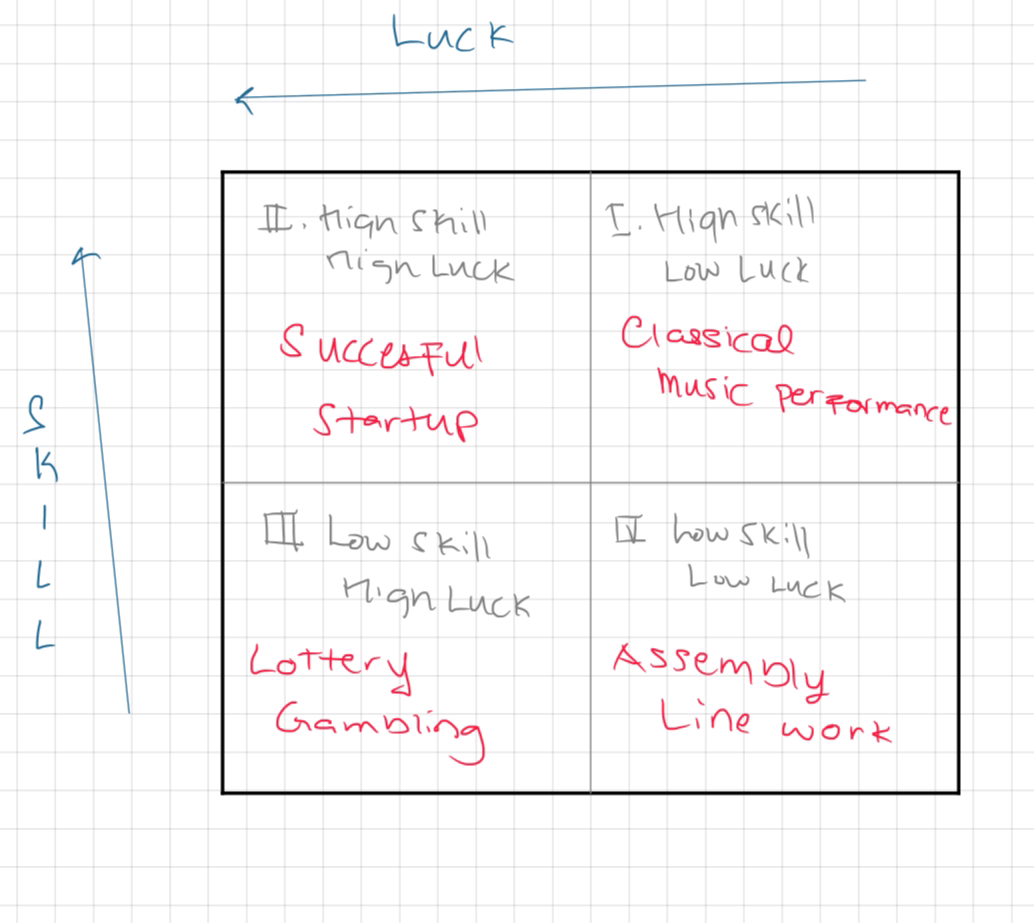
\includegraphics[width=0.5\textwidth]{2x2.png}
  \caption{2X2 Luck - Skill Matrix}
  \label{fig:example}



\easysubproblem{[EC] Why do you think Billing's algorithms (and other algorithms like his) are not very good at no-limit hold em? I can think of a couple reasons why this would be.}\spc{2} \\ 
Billing's algorithms, like many others, may struggle  in no limit hold'em due to the game's complexity and need for nuanced decision-making. No-limit hold'em involves not only strategic betting but also bluffing, hand reading, and adjusting to opponent's play styles, which are challenging for algorithms to accurately model. Additionally, the immense number of possible game states in no-limit hold'em makes it difficult for algorithms to explore and evaluate all options effectively, leading to sub optimal decisions.

\easysubproblem{Do you agree with Silver's description of what makes people successful (pp326-327)? Explain.}\spc{2} \\ 
I agree with Silver's take on the role that luck plays into the reasons for success. It is true that people need to be skilled enough as well as disciplined enough to keep working and improving but the opportunity to rise is the biggest factor. The best programming students could exist everywhere but if they don't apply for jobs they may never be discovered. The converse is true a lot of unskilled developers are out there due to opportunities such as referrals that put them in front of more deserving people. CS Students can study and code all day receiving the highest grades and creating the coolest projects but if they dont take the time to network and allow themselves to become a desirable candidate / applicant, they will forever live in the shadows to wonder why they have no jobs. 

\easysubproblem{Silver brings up an interesting idea on p328. Should we remove humans from the predictive enterprise completely after a good model has been built? Explain}\spc{2} \\ 
This  is a classical case of Human vs Automation. Like all things there are trade offs. In this specific domain for predictive enterprise, Humans could be removed from the entire mathematical computation but for analysis I think humans are still required. Yes a model can also analyze and interpret the data using Large language models like CHATGPT but If everything is fully automated that can assume stationarity. Things may change and the model may be inaccurate with time. Second the model itself maybe good but bias, a human interpretting the results could act as a checks and balance between the model the same way that a model may remove a human's bias. Models are also just machines that spit out numbers, they have no ethics. To remove a human from automation may prevent the generalization of factors that the model did not consider. Overall I think humans can be removed in some aspects but humans are still necessary in analysing and interpretting the models results. It is a human's job to validate the model and its results because at the end of the day models are just tools. 

\easysubproblem{According to Fama, using the notation from this class, how would explain a mutual fund that performs spectacularly in a single year but fails to perform that well in subsequent years?}\spc{1} \\ 
To explain using the context of our class the reason that a mutual fund that performs well but is unable to replicate its success could be a victim of high bias that year. It may just be that at that specific year it really did well making people believe in that mutual fund. Another thing is maybe the analysts assumed stationarity that every year forward it would perform well which is never usually the case. 

\easysubproblem{Did the Manic Momentum model validate? Explain.}\spc{1} \\ \\
The Manic Momentum model, discussed in Nate Silver's book "The Signal and the Noise," relates to the prediction of financial markets, particularly focusing on stock prices and their movements. The concept of "Manic Momentum" refers to the idea that stock prices can exhibit momentum that is, trends in stock prices can persist in one direction for a period of time before possibly reversing. It was validated through several ways such as \textbf{Market efficiency}, \textbf{Volatility}, \textbf{Empirical Evidence, } etc. We can conclude that the Manic momentum does capture some aspects of real-world market dynamics, especially thing that persist in the short term. 


\easysubproblem{Are stock market bubbles noticable while we're in them? Explain.}\spc{1} \\ \\
Noticing stock market bubbles while we are in them is relatively hard because during a bubble, market sentiment is often overwhelmingly positive, which can cloud judgment. Investors may become overly optimistic about the continued growth and ignore sings of overvaluation. The rapid increase could also encourage other investors to ride the wave, this is called herd mentality. It also isn't that simple to label and identify a bubble since there is no precise or universally accepted definition of what a bubble is, which makes it hard to identify one until after it has burst. 

\easysubproblem{What is the implication of Shiller's model for a long-term investor in stocks?}\spc{1} \\ \\
For long-term investors, Shiller’s model implies that when stock valuations are high relative to historical earnings, future returns are likely to be lower. Therefore, adjusting asset allocations based on valuation levels and taking a more conservative stance when valuations are high and might improve long-term investment outcomes. 

\easysubproblem{In lecture one, we spoke about \qu{heuristics} which are simple models with high error but extremely easy to learn and live by. What is the heuristic Silver quotes on p358 and why does it work so well?}\spc{1} \\ \\

In Nate Silver's book,  he discusses the heuristic of assuming continuity over change in uncertain situations. Specifically, he mentions, "When something is new or hard to understand, bet that the trend will continue rather than that it will reverse." This heuristic simplifies decision-making in complex situations by suggesting that existing trends are likely to persist. In many areas, once a trend is established, it often continues due to underlying forces. For example, in economics, markets that are rising or falling tend to continue to do so. Systems, whether they are natural, economic, or social, typically have inherent resistance to change. It requires a lot more forces to change which is not usually common. 

\easysubproblem{Even if your model at predicting bubbles turned out to be good, what would prevent you from executing on it?}\spc{1} \\ \\ 
Even with a reliable model for predicting financial bubbles, practical challenges like the difficulty of timing the market accurately, psychological pressures, market impact of large trades, regulatory constraints, financial limitations, counterparty risks, and potential feedback loops can all hinder the successful execution of trading strategies based on such predictions. These factors make it complex to act on theoretical models in the dynamic and often unpredictable real-world financial markets.

\easysubproblem{How can heuristics get us into trouble?}\spc{5} \\ \\ 
Heuristics simplify decision-making but can lead to problems such as overgeneralization, embedded cognitive biases, resistance to new information, misjudgment of probabilities, and an illusion of validity. They can also result in stereotyping and neglecting the complexity of situations, potentially leading to discriminatory practices and oversimplified solutions to complex problems. These limitations highlight the need for careful management and critical evaluation of heuristic-based decisions.

\end{enumerate}

\newpage 
\problem{These are some questions related to polynomial-derived features and logarithm-derived features in use in OLS regression.}

\begin{enumerate}

\intermediatesubproblem{What was the overarching problem we were trying to solve when we started to introduce polynomial terms into $\mathcal{H}$? What was the mathematical theory that justified this solution? Did this turn out to be a good solution? Why / why not?}\spc{3} \\ \\ 
The issue that occurs was when the data is overly complex that our candidate set $\mathcal{H}$ was unable to find any set of functions that could fully grasp the complexity of $\mathcal{D}$. For example if there is an upward curve trend within the data and our $\mathcal{H}$ only consisted of linear functions we would incur a lot of mispecification error.  The solution we introduced was resorting to higher term polynomials. Since the computer just takes input we can trick it by utilizing higher level polynomials that are still in the form of linear functions. It is also convenient mathematically because OLS will still be a viable option despite making the equation more complex. 

\intermediatesubproblem{We fit the following model: $\yhat = b_0 + b_1 x + b_2 x^2$. What is the interpretation of $b_1$? What is the interpretation of $b_2$? Although we didn't yet discuss the \qu{true} interpretation of OLS coefficients, do your best with this.}\spc{4} \\ \\ 
$b_1$ is the linear coefficient of the model. It represents the linear effect of the predictor variable x on the response variable  $\yhat$. $b_2$ is the coefficient of the quadratic term $x^{2}$. It quantifies the curvature effect of x on $\yhat$.  
 
\hardsubproblem{Assuming the model from the previous question, if $x \in \mathcal{X} = \bracks{10.0, 10.1}$, do you expect to \qu{trust} the estimates $b_1$ and $b_2$? Why or why not?}\spc{7} \\ \\ 
Given the narrow range of \textit{x}, estimates $b_1$ and $b_2$ should be treated with caution. They are likely to be very sensitive to the specific dataset and might not generalize well outside this narrow window. If the model's purpose is to make predictions within a similar narrow range or to understand the relationship in this specific interval, the estimates might be useful. However, for broader applications or predictions over a more extensive range of \textit{x}, these coefficients may not provide reliable or trustworthy insights. Additional data covering a broader range of \textit{x} values would be beneficial to test the robustness and applicability of the model. 
 
\newpage

\hardsubproblem{We fit the following model: $\yhat = b_0 + b_1 x_1 + b_2 \natlog{x_2}$. We spoke about in class that $b_1$ represents loosely the predicted change in response for a proportional movement in $x_2$. So e.g. if $x_2$ increases by 10\%, the response is predicted to increase by $0.1 b_2$. Prove this approximation from first principles.}\spc{6} \\ \\ 

The explanation provided shows how a percentage change in $x_2$ affects the response variable $\yhat$ in the model $\yhat = b_0 + b_1 x_1 + b_2 \natlog{x_2}$. Here’s a summary of the key steps: 

\begin{enumerate}
    \item \textbf{Model Derivation}: The model suggests that changes in $x_2$ through the natural logarithm of $x_2$.
    \item \textbf{Rate of Change Calculation:} The derivative of $\yhat$ with respect to  $x_2$ is $b_2$/$x_2$. This derivative indicates how much $\yhat$ changes for a small unit change in $x_2$
    \item \textbf{Effect of Percentage Change}: When $x_2$ increases by a percentage \textit{p}\%, $x_2$ changes to $x_2$(1+p/100). Using the properties of logarithms, the change in $\yhat$(Δ$\yhat$) can be estimated by $b_2$ln(1+p/100).
    \item \textbf{Approximation for Smal}l \textit{p}: For small percentage changes \textit{p}, the logarithm ln⁡(1+p/100) can be approximated by \textit{p}/100 using the Taylor expansion. This results in (Δ$\yhat$ $\approx $ $b_2$(p/100)
    \item \textbf{Interpretation} : Thus, if $x_2$ increases by 10\%, the increase in $\yhat$ is approximately 0.1$b_2$. This calculation shows how the model predicts a proportional change in the response based on a percentage change in $x_2$ 
\end{enumerate}
 

\easysubproblem{When does the approximation from the previous question work? When do you expect the approximation from the previous question not to work?}\spc{4} \\ \\ 
The approximation $\ln\left(1 + \frac{p}{100}\right) \approx \frac{p}{100}$ is very useful for quick calculations and is often sufficiently accurate for practical purposes when dealing with small changes. However, for larger changes, for systems where precision is paramount, or where the response is highly non-linear, more robust methods of analysis should be considered. The decision to use such an approximation should be guided by the context and the acceptable level of error in the specific application.


\intermediatesubproblem{We fit the following model: $\natlog{\yhat} = b_0 + b_1 x_1 + b_2 \natlog{x_2}$. What is the interpretation of $b_1$? What is the \emph{approximate} interpretation of $b_2$? Although we didn't yet discuss the \qu{true} interpretation of OLS coefficients, do your best with this.}\spc{2} \\ \\ 

In summary, $b_1$ quantifies the multiplicative effect on $\hat{y}$ for a one-unit change in $x_1$ and can be interpreted straightforwardly as an exponential effect. The coefficient $b_2$, on the other hand, represents the elasticity of $\hat{y}$ with respect to $x_2$, indicating how much $\hat{y}$ changes in percentage terms in response to a 1\% change in $x_2$. These interpretations are essential for understanding the impact of variables in models where logarithmic transformations are employed, providing insights into the proportional and relative effects of changes in predictor variables.


\easysubproblem{Show that the model from the previous question is equal to $\yhat = m_0 m_1^{x_1} x_2^{b_2}$ and interpret $m_1$.}\spc{2} \\ \\ 

Step 1: Original Model : \\ 
$\[
\ln(\hat{y}) = b_0 + b_1x_1 + b_2 \ln(x_2)
\]$ 

Step 2: Exponentiate Both Sides \\ 
$\[
\hat{y} = e^{b_0 + b_1x_1 + b_2 \ln(x_2)}
\]$

Step 3: Simplify  \\
Utilize identity $e^{ln(a)} = a $ : \\
$
\yhat = e^{b_0} \cdot e^{b_1 x_1} \cdot x_2^{b_2}

$

\\ 
Step 4: Define Constants \\ 
Define $m_0 = e^{b_0}$ and $m_1 = e^{b_1}$ \\ 
$\yhat = m_0 \cdot m_1^{x_1} \cdot x_2^{b_2}$ \\
\end{enumerate}


\newpage
\problem{These are some questions related to extrapolation.}

\begin{enumerate}

\easysubproblem{Define extrapolation and describe why it is a net-negative during prediction.}\spc{3} \\ \\ 
Extrapolation is when you predict future events based on trends from existing data that go beyond the range you originally studied. For example, if you have only seen the sales data for the first six months of the year, and you try to guess what will happen at the end of the year, you're extrapolating. This method can be risky and often produces inaccurate results because it assumes that current trends will continue unchanged. For instance, if you noticed more ice cream sales in the early summer months and extrapolated that this would continue, you might predict extremely high sales for December, which is unlikely due to the colder weather reducing demand for ice cream.

\easysubproblem{Do models extrapolate differently? Explain.}\spc{3} \\ \\ 
Yes, different models extrapolate differently based on how they are built and what they assume about the data. For instance, a simple model might assume that sales grow by a fixed amount each month, so if you tell it that sales have been increasing from January to June, it might just continue that trend into the future. More complex models might consider other factors like seasonal changes or economic conditions, which could lead to different predictions for the future. Each model has its own way of handling data outside of its original range, leading to varying results when extrapolating.

\easysubproblem{Why do polynomial regression models suffer terribly from extrapolation?}\spc{3} \\ \\ 
Polynomial regression models suffer terribly from extrapolation because they follow curves that can change dramatically outside the range of data they were trained on. For example, if a polynomial model is used to fit a set of points that rise slowly, it might curve sharply upward or downward when trying to predict values beyond those points. This makes the model very unreliable for predicting outside its original data set, as it might give extreme values that don’t make sense with real-world behavior.


\end{enumerate}
\newpage
%
%\problem{These are some questions related to polynomial-derived features and logarithm-derived features in use in OLS regression.}
%
%\begin{enumerate}
%
%\intermediatesubproblem{What was the overarching problem we were trying to solve when we started to introduce polynomial terms into $\mathcal{H}$? What was the mathematical theory that justified this solution? Did this turn out to be a good solution? Why / why not?}\spc{3}
%
%\intermediatesubproblem{We fit the following model: $\yhat = b_0 + b_1 x + b_2 x^2$. What is the interpretation of $b_1$? What is the interpretation of $b_2$? Although we didn't yet discuss the \qu{true} interpretation of OLS coefficients, do your best with this.}\spc{4}
%
%\hardsubproblem{Assuming the model from the previous question, if $x \in \mathcal{X} = \bracks{10.0, 10.1}$, do you expect to \qu{trust} the estimates $b_1$ and $b_2$? Why or why not?}\spc{7}
%
%\hardsubproblem{We fit the following model: $\yhat = b_0 + b_1 x_1 + b_2 \natlog{x_2}$. We spoke about in class that $b_1$ represents loosely the predicted change in response for a proportional movement in $x_2$. So e.g. if $x_2$ increases by 10\%, the response is predicted to increase by $0.1 b_2$. Prove this approximation from first principles.}\spc{7}
%
%\easysubproblem{When does the approximation from the previous question work? When do you expect the approximation from the previous question not to work?}\spc{2}
%
%\intermediatesubproblem{We fit the following model: $\natlog{\yhat} = b_0 + b_1 x_1 + b_2 \natlog{x_2}$. What is the interpretation of $b_1$? What is the interpretation of $b_2$? Although we didn't yet discuss the \qu{true} interpretation of OLS coefficients, do your best with this.}\spc{3}
%
%\easysubproblem{Show that the model from the previous question is equal to $\yhat = m_0 m_1^{x_1} x_2^{b_2}$ and interpret $m_1$.}\spc{2}
%
%\end{enumerate}

\problem{These are some questions related to the model selection procedure discussed in lecture.}

\begin{enumerate}

\easysubproblem{Define the fundamental problem of \qu{model selection}.}\spc{6} \\ \\ 
The fundamental problem of model selection is that each hyperparameter, each algorithm, the amount of data you use, etc, will all produce different models. There is a multitude of models you can come up with. The problem is how do we know if we obtained the best model possible that generalizes well on unseen data. We would need a model that is closest to f.

\easysubproblem{Using two splits of the data, how would you select a model?}\spc{8} \\\\
Splitting the dataset into two implies that the majority off it will be used to train and the remained will be used for testing which we would give you a rough estimate on how well the model will do. 

\easysubproblem{Discuss the main limitation with using two splits to select a model.}\spc{3} \\ \\ 
The test set could only be used once. If you utilize it multiple times your model can over fit. The dilemma is how do i make adjustments to my model while being able to have honest metrics. 

\easysubproblem{Using three splits of the data, how would you perform model selection?}\spc{3} \\ \\ 
Three splits introduce a new split called validation set. This is an intermediarry step that we is part of the training set. We could train the model and proxy-test it using the validation set which we can use again and again, with the possibility of overfitting to the validation set increases if you are not careful, before testing on the actual test set. This allows more flexibility during model selection. 

\easysubproblem{How does using both inner and outer folds in a double cross-validation nested resampling procedure improve the model selection procedure?}\spc{3} \\ \\ 
Using inner and outer folds means that the inner fold is used for tuning the hyperparameter/ selecting the best model and the outer fold is used to show how well the
model selected from the inner fold will perform on unseen data. As the name implies,
this is cross-validating and will help in improving the model selection procedure.

\easysubproblem{Describe how $g_{\text{final}}$ is constructed when using nested resampling on three splits of the data.}\spc{5} \\ \\ 
When using nested resampling on three splits, the inner fold determines the best
model/ hyperparameter. The selected model/hyperparameters from each inner fold
are retrained on the entire outer fold training set. The gfinal is the final model that is
ready to be used on unseen data

\easysubproblem{Describe how you would use this model selection procedure to find hyperparameter values in algorithms that require hyperparameters.}\spc{3} \\ \\ 
Model selection for models that have hyperparameters in their algorithms could be done iteratively. For example x is a hyperparameter. We could have give x a range for example 1-100. Iteratively train, test, collect error metrics. Iterative checking could be done by a foor loop. Once we search all possible outcomes we can just select the combination of hyperparemeters that produced the lowest errors. 

\hardsubproblem{Given raw features $x_1, \ldots, x_{p_{raw}}$, produce the most expansive set of transformed $p$ features you can think of so that $p \gg n$.}\spc{3} \\ \\ 
To produce the most expansive set we could Generate all polynomial combinations of the features up to a certain degree. For example, with two features $x_1$ and $x_2$, and up to degree 2, you'd create more complex versions of the raw features. The next thing we can do beyond simple polynomial terms is to include interaction between terms for different features. 

\easysubproblem{Describe the methodology from class that can create a linear model on a subset of the transformed featuers (from the previous problem) that will not overfit.}\spc{10} \\ \\ First we generate the expanded set of features using the transformations discussed such as polynomial expansion and interaction of terms. Then feature selection. We utilize filter methods to select features that have a strong relationship with the target variable. 

\end{enumerate}

\newpage

\problem{These are some questions related to the CART algorithms.}

\begin{enumerate}
\easysubproblem{Write down the step-by-step $\mathcal{A}$ for regression trees.}\spc{7} \\ \\ 

\item Start at the root : Begin with all the training data at the root node
\item Feature selection : For each feature, attempt to find the best split that divides the data into two groups. Select the split with the lowest MSE.
\item Actually split the data
\item Create a leaf node : Establish a stopping criteria. Assign model prediction to leaf nodes. 
\item Once you identify the best rebuild the entire tree with the most optimal hyperparameters (Height) and best features. 

\hardsubproblem{Describe $\mathcal{H}$ for regression trees. This is very difficult but doable. If you can't get it in mathematical form, describe it as best as you can in English.}\spc{7} \\ \\ 
H for regression trees is every possible combination of features in D as indicators functions. There could be infinite ways to combine a trees predictors especially as n grows larger. 

\intermediatesubproblem{Think of another \qu{leaf assignment} rule besides the average of the responses in the node that makes sense.}\spc{3} \\ \\ 
In regression trees, choosing a suitable leaf assignment rule is crucial for the model's performance. Besides using the average of the responses in the node, another effective rule for assigning values to leaf nodes is the median of the responses in the node. This allows us to be more robust since median is less sensitive to outliers compared to the mean. 

\intermediatesubproblem{Assume the $y$ values are unique in $\mathbb{D}$. Imagine if $N_0 = 1$ so that each leaf gets one observation and its $\yhat = y_i$ (where $i$ denotes the number of the observation that lands in the leaf) and thus it's very overfit and needs to be \qu{regularized}. Write up an algorithm that finds the optimal tree by pruning one node at a time iteratively. \qu{Prune} means to identify an inner node whose daughter nodes are both leaves and deleting both daughter nodes and converting the inner node into a leaf whose $\yhat$ becomes the average of the responses in the observations that were in the deleted daughter nodes. This is an example of a \qu{backwards stepwise procedure} i.e. the iterations transition from more complex to less complex models.}\spc{5} \\ \\ 
Steps: \\ 
\textbf{Start Fully Grown} : Begin with a tree where each data point in your dataset forms a leaf. Each leaf’s prediction is just the target value of that single data point.

\textbf{Check for Pruning Candidates}: Look through all the internal nodes of the tree. Identify any internal node where both children are leaves (these nodes are candidates for pruning).

\textbf{Prune a Node:} For each candidate node, consider the two daughter leaves. Remove these leaves and turn the internal node into a new leaf.
The prediction for this new leaf becomes the average of the target values from the two removed leaves.

\textbf{Iterate:} Repeat the process: After each pruning, re-evaluate the tree to find new pruning candidates.
Continue pruning until no further internal nodes have two leaf children, or until you reach a predetermined stopping criterion (like a desired number of leaves).

\textbf{Result: }The end result is a simpler tree that is less likely to overfit the data since it generalizes by averaging responses over more observations per leaf.


\hardsubproblem{Provide an example of an $f(\x)$ relationship with medium noise $\delta$ where vanilla OLS would beat regression trees in oos predictive accuracy. Hint: this is a trick question.}\spc{1} \\ \\ 
 If the actual underlying relationship between the predictors and the response is linear, OLS, which directly models this linearity, would likely have better predictive accuracy. This is because it efficiently estimates the parameters with methods that minimize the sum of squared errors, directly targeting the core of the linear relationship. OTHER THAN THAT REGRESSION TREES IS KING! 

\easysubproblem{Write down the step-by-step $\mathcal{A}$ for classification trees. This should be short because you can reference the steps you wrote for the regression trees in (a).}\spc{4} \\ \\ 

a. Start at the root : Begin with all the training data at the root node
b. Feature selection : For each feature, attempt to find the best split that divides the data into two groups. Select the split with the lowest \textbf{missclassification error}.
c. Actually split the data
d. Create a leaf node : Establish a stopping criteria. Assign model prediction to leaf nodes. 
e. Once you identify the best rebuild the entire tree with the most optimal hyper parameters (Height) and best features. 

\hardsubproblem{Think of another objective function that makes sense besides the Gini that can be used to compare the \qu{quality} of splits within inner nodes of a classification tree.}\spc{6} \\ \\ 
Entropy. This measure is a fundamental concept from information theory and is particularly effective in the context of decision trees for classification, often used in the construction of C4.5 trees, a successor of the basic ID3 algorithm. 


\end{enumerate}







\end{document}






